\section*{Discussion}

\noindent In this study we quantify essential characteristics of \textit{Ae. aegypti} larval behavior that are crucial for the development of future studies. Further, we identify previously unknown behaviors that highlight the unique evolutionary history and developmental biology of these disease vector mosquitoes. First, we show that larvae perceive microbial RNA as a foraging attractant, but do not respond to several olfactory cues that attract adult \textit{Ae. aegypti} for oviposition. Second, we demonstrate that \textit{Ae. aegypti} larvae use chemokinesis, rather than chemotaxis, to navigate with respect to chemical sources. Using data-driven computational modeling, we further show that chemokinesis is superior to chemotaxis in avoiding repellents in ecologically relevant larval habitat sizes. Finally, we use experimental observations and computational analyses to demonstrate that larvae respond to starvation pressure by changing their behavior to increase the probability of finding a scarce food source without compromising their ability to successfully avoid repellents. 

\begin{figure}[t!]
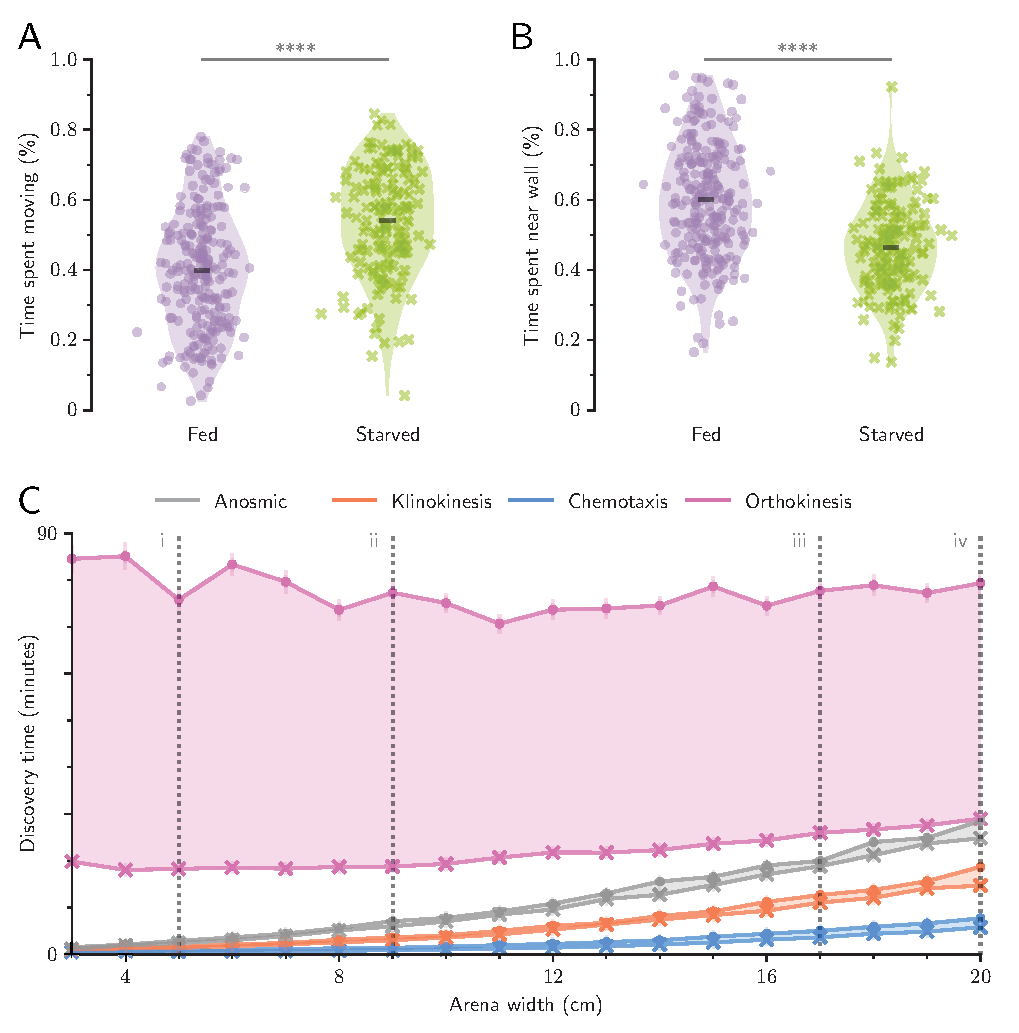
\includegraphics[width=\textwidth]{Figures/images/6.eps}
 \caption{\textbf{ Starved \textit{Ae. aegypti} optimize exploration behavior to increase the probability of finding food.} A: Starved larvae spend significantly more time exploring the arena than fed larvae. B: Starved larvae spend significantly less time within one body length of an arena wall. (A,B) Violin plot. Dots are the means for each individual, and black bar is the mean across all individuals (n>168 per treatment); asterisks denote p<0.0001 (Welch's t-test).  C: Simulated chemokinetic larvae using empirical data from starved animals found the food source consistently faster than the same model using data from fed animals. Shaded regions show difference between fed (X markers) and starved (dots) simulations (mean ${\pm}$ standard error). Dashed grey lines correspond to ecologically relevant habitat sizes described in Table 2. 
}
\end{figure}

These results are fascinating from both a developmental biology and disease prevention perspective. In their adult form and during flight, \textit{Ae. aegypti} exhibit an odor-tracking behavior termed odor-conditioned optomotor anemotaxis, where encounter with an odor gates an upwind surge in the wind direction \cite{Van_Breugel2015-an}. In this behavior, successive odor encounters are necessary to prolong the upwind flight towards the upwind odor source, and the gradient information is not necessary to elicit the upwind responses. In other insects, such as \textit{D. melanogaster}, while walking but not flying, these animals exhibit a form of chemotactic behavior where bilateral comparisons are made between antenna \cite{Gaudry2012-li}. It remains unclear whether walking adult \textit{Ae. aegypti} may also exhibit similar chemotactic behaviors, but given the differences between adult and larval responses, this species may provide an excellent developmental model to  identify neurobiological pathways integral to olfactory navigation. Previous studies on mosquito larvae can further contextualize our results and provide additional insight. Unlike \textit{Ae. aegypti}, \textit{Anopheles gambiae} mosquito larvae prefer both indole and o-cresol, in addition to many other olfactory stimuli \cite{Xia2008-hw}. The stark differences in larval chemosensory behavior mirror the many differences observed between the adults of these two species \cite{Bohbot2007-nw}, and suggests that studies should be cautious of generalizing among disease vector mosquitoes.

Although adult \textit{Ae. aegypti} feeding is regulated by ATP perception \cite{Galun1985-we}, we are unaware of other work demonstrating RNA attraction in \textit{Ae. aegypti} larvae. In our state-dependent preference experiments, we investigate the ecological basis of larval RNA attraction, and propose that RNA may function as a foraging indicator in the larval environment. Although the receptor responsible for RNA detection is unknown, work in \textit{D. melanogaster} suggests that a gustatory or ionotropic receptor may be more likely candidates than an olfactory receptor. In addition, an earlier study demonstrated that olfactory deficient (\textit{orco -/-}) \textit{Ae. aegypti} larvae showed no defects in attraction to food or avoidance of quinine \cite{Bui2018-iq}. Taken together, our results support the hypothesis that sensory information gained from gustatory or ionotropic receptors may be more integral to larval chemosensation than olfactory receptors. Further, larval attraction to RNA suggests that the importance of nucleotide phagostimulation is preserved throughout a mosquito's life cycle, from larval foraging to adult blood engorgement and oviposition.

Our computational experiments suggest an ecological basis for the lack of chemotaxis in \textit{Ae. aegypti} larvae. Although our experiments showed that chemotaxis is superior to chemokinesis in foraging, chemokinesis surpassed chemotaxis, klinokinesis and anosmic strategies in avoiding repellents. This suggests that the role of chemosensation in larvae is primarily tuned toward aversive responses. Indeed, known characteristics of larval physiology support this idea. Although larvae can survive for up to a week without food, they quickly succumb to toxic bacterial byproducts \cite{Christophers1960-xf,Floore2006-si}. We propose that \textit{Ae. aegypti} larvae combat starvation pressure primarily through physiological adaptations such as fat stores, and resist toxins in the environment through chemosensory behaviors optimized for avoiding repellents. 

Our study also raises a number of comparative questions that could be addressed in future research. For instance, is chemokinesis in mosquito larvae associated with generalized spatial restriction, or with human association and man-made containers in particular? Future studies could compare chemotactic ability in other spatially constrained mosquitoes, such as \textit{Toxorhynchites} (which inhabit tree holes) or \textit{Aedes albopictus} (another container-breeding mosquito) \cite{Hoel2011-er}, to species that oviposit in larger bodies of water such as \textit{Aedes togoi} (marine rock pools) or opportunistic species such as \textit{Culex nigripalpus} that oviposit in a wide range of habitat sizes \cite{Hoel2011-er,Bentley1989-ct}. Additionally, computational modeling of fluid dynamics and larval movement may help determine whether chemotaxis is physically challenging in small, man-made environments. Shallow gradients in small containers may diffuse too quickly to be used as a reliable chemical signal - particularly considering our results showing that larval movement significantly increases stimulus diffusion \cite{Hein2016-in}. 

Synanthropic mosquitoes are increasingly important to global health as urbanization progresses: Currently over half of all humans live in urban environments, and this proportion is only expected to increase \cite{Goddard2010-wf}. Adaptations that facilitate human cohabitation, like specialized larval foraging strategies, are vital to our understanding of mosquito behavior and success as a disease vector \cite{Gubler2014-no}. 


